\documentclass[a4paper,11pt]{article}
\usepackage{amsmath,amsthm,amsfonts,amssymb,amscd,amstext,vmargin,graphics,graphicx,tabularx,multicol} 
\usepackage[francais]{babel}
\usepackage[utf8]{inputenc}  
\usepackage[T1]{fontenc} 
\usepackage{pstricks-add,tikz,tkz-tab,variations}
\usepackage[autolanguage,np]{numprint} 

\setmarginsrb{1.5cm}{0.5cm}{1cm}{0.5cm}{0cm}{0cm}{0cm}{0cm} %Gauche, haut, droite, haut
\newcounter{numexo}
\newcommand{\exo}[1]{\stepcounter{numexo}\noindent{\bf Exercice~\thenumexo} : \marginpar{\hfill /#1}}
\reversemarginpar


\newcounter{enumtabi}
\newcounter{enumtaba}
\newcommand{\q}{\stepcounter{enumtabi} \theenumtabi.  }
\newcommand{\qa}{\stepcounter{enumtaba} (\alph{enumtaba}) }
\newcommand{\initq}{\setcounter{enumtabi}{0}}
\newcommand{\initqa}{\setcounter{enumtaba}{0}}

\newcommand{\be}{\begin{enumerate}}
\newcommand{\ee}{\end{enumerate}}
\newcommand{\bi}{\begin{itemize}}
\newcommand{\ei}{\end{itemize}}
\newcommand{\bp}{\begin{pspicture*}}
\newcommand{\ep}{\end{pspicture*}}
\newcommand{\bt}{\begin{tabular}}
\newcommand{\et}{\end{tabular}}
\renewcommand{\tabularxcolumn}[1]{>{\centering}m{#1}} %(colonne m{} centrée, au lieu de p par défault) 
\newcommand{\tnl}{\tabularnewline}

\newcommand{\bmul}[1]{\begin{multicols}{#1}}
\newcommand{\emul}{\end{multicols}}

\newcommand{\trait}{\noindent \rule{\linewidth}{0.2mm}}
\newcommand{\hs}[1]{\hspace{#1}}
\newcommand{\vs}[1]{\vspace{#1}}

\newcommand{\N}{\mathbb{N}}
\newcommand{\Z}{\mathbb{Z}}
\newcommand{\R}{\mathbb{R}}
\newcommand{\C}{\mathbb{C}}
\newcommand{\Dcal}{\mathcal{D}}
\newcommand{\Ccal}{\mathcal{C}}
\newcommand{\mc}{\mathcal}

\newcommand{\vect}[1]{\overrightarrow{#1}}
\newcommand{\ds}{\displaystyle}
\newcommand{\eq}{\quad \Leftrightarrow \quad}
\newcommand{\vecti}{\vec{\imath}}
\newcommand{\vectj}{\vec{\jmath}}
\newcommand{\Oij}{(O;\vec{\imath}, \vec{\jmath})}
\newcommand{\OIJ}{(O;I,J)}


\newcommand{\reponse}[1][1]{%
\multido{}{#1}{\makebox[\linewidth]{\rule[0pt]{0pt}{20pt}\dotfill}
}}

\newcommand{\titre}[5] 
% #1: titre #2: haut gauche #3: bas gauche #4: haut droite #5: bas droite
{
\noindent #2 \hfill #4 \\
#3 \hfill #5

\vspace{-1.6cm}

\begin{center}\rule{6cm}{0.5mm}\end{center}
\vspace{0.2cm}
\begin{center}{\large{\textbf{#1}}}\end{center}
\begin{center}\rule{6cm}{0.5mm}\end{center}
}



\begin{document}
\pagestyle{empty}
\titre{Interrogation: Calcul littéral }{Nom :}{Prénom :}{Classe}{Date}


\exo{2} Réduire les expressions suivantes : 

\bmul{2}

$M = -7 +5x+12x^{2}  -21 +7x^{2}$\\
\reponse[3]\\


\columnbreak

$T = (-7) \times 2 \times t \times t -3 \times 5t +9 \times t$\\
\reponse[3]\\

\emul

\exo{5} Développer et réduire les expressions suivantes:


\bmul{2}

$R = 8(7x + 9)$\\
\reponse[4]\\

$V = (x-6)(2-3x)$\\
\reponse[6]\\

\columnbreak

$G = -7x(4x-2)$\\
\reponse[4]\\


$P = (2-x)(x+4)+5(-x+2)$\\
\reponse[7]\\


\emul


\exo{3}

\q Soient $ D = (12x + 3)(2x - 7) -(2x -7)^{2} $ et $ L = x^{3} - 4 x^{2} -x+44$\\

\qa Calculer la valeur de \textbf{l'expression D} pour $x=0$.\\
\reponse[7]\\

\newpage

\qa Calculer la valeur de \textbf{l'expression L} pour $x=-3$.\\
\reponse[7]\\

\q \textbf{Vrai ou faux.} Justifier votre réponse par un calcul.\\
\begin{center}
Pour $b=\dfrac{1}{2}$, $4b^{2} + 1 =2$
\end{center}
\reponse[7]\\

\exo{} BONUS

Les figures ci-dessous ont-elles le même périmètre ?\\
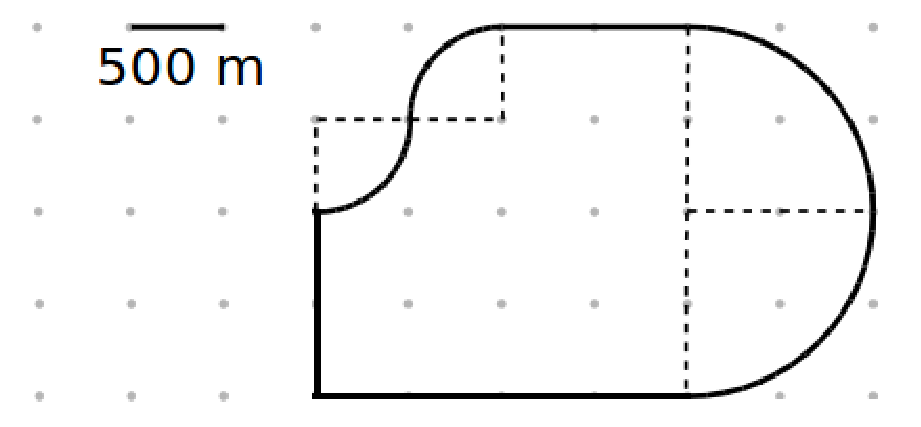
\includegraphics[scale=0.7]{perimetre.eps} \\
\reponse[4]\\

\end{document}
